

\chapter{Insight\label{ch:insight}}

\section{Introduction}
 {

  Prior to any change to the built environment, is the full understanding and evaluation of the current state of the city. Gaining meaningful insights can highlight places, policies, or behaviors in need for transformation, so that decision-makers can better focus their resources and efforts. As a complex systems of systems \cite{Batty2009}, the many different layers of information in the city are challenging to comprehend. Narrowing the spectrum of possible observations, through methodical data collection, accurate analysis, and clear representation, is a critical step towards a productive planning discourse \cite{banerjee2011companion}. This chapter discusses how CityScope is used to expose the current state of the city, focusing on data aggregation, analysis, and representation.


  \subsection{From Static Data to Urban Dynamics}

  {
      In recent decades, many data-driven methodologies emerged to provide empirical assessments of urban performance \cite{Inostroza2015, hillier1987ideas}. In the 1970's, `Space Syntax' was proposed as a set of analytical tools to interpret the \textit{``ordering of space into relational systems''} \cite{Hillier1993}, using quantitative analysis to infer the performance of spatial networks. At the time, data accuracy and geometric-spatial limitations confined the results to generalized outputs \cite{herold2005role}. Today, the abundance of urban data and the advancement of spatial analytics greatly improve the resolution and accuracy of these evaluations \cite{Batty2000}. Nevertheless, urban performance cannot be solely interpreted by analyzing urban-form: the quality of a place is a joint artifact of physical places and the society which occupies them \cite{lynch1984good}. To associate form with behavior, Lynch proposed \textit{``Performance Dimensions''}: a set of spatial and experiential urban features, bridging the gap between form and usage. Along the same lines, Gehl suggested metrics to reflect the social impacts of a public space and the quality of life of its users \cite{gehl2013study}. Today, with the growing ubiquity of tracking devices and slew of behavioral data, it is possible to analyze the `real-time city', as a useful design and planning apparatus \cite{ Ratti2006, Kitchin2014, Batty2013}.
  }

  \subsection{Urban Dynamics: Mobility and Behavior}\label{subsec:andorra-data-observatory-mobility}

  {
      The growth of Location Based Services (LBS) motivated the research of the city's `beating pulse' \cite{Becker2011}. In recent decades, mobile devices became the major way to observe human dynamics, behavioral patterns, mobility, large public events, and emergencies \cite{Blondel2015, Calabrese2014, Reades2007, gonzalez2008understanding, Deville2014, Berlingerio2013}. Other location sensing technologies, such as GPS, radio frequency identification, cameras, or activity sensors, are all limited in their spatial capacity, the need for active user-interaction (`opt-in'), and complexity of data extraction.
      \newline
      Studies in Belgium, UK, Ivory Coast, and Spain showed correlations between the spatial form of cities, the distribution of their activity `hot-spots', and the degree of interaction between different cellular users \cite{Blondel2015, Louail2014}. Similarly, spatial-temporal regularity within behavioral trajectories was found in mobile phone users, suggesting that individuals can be clustered into different groups based on their behavioral patterns \cite{Song2010}. Others have used LBS to characterize individual trajectories across the city, showing collective behavior and `flocking' patterns \cite{Ratti2006, DecodingtheCity}. Despite the promise of location data for urban analytics, challenges still exist in data accuracy, temporal resolution, and bias.
  }

  \subsection{Limitations of LBS}

  {
      In the past, LBS limitations in data quantity, reliability, and accuracy have forced spatial generalization and limited outcomes \cite{candia2008uncovering}. In many cases, Call Detail Records (CDR) data were the prevailing LBS in use \cite{jiang2017activity}. CDR provide usage history, cell tower ID, and approximate coverage region of each base-station, which together are used to estimate the location-time of users. However, CDRs suffer from low temporal and spatial resolution, since location information is only provided at the cell tower level and updates are only received when the device is in use, such as during calls or text \cite{Calabrese2014}. Moreover, studies have shown that CDRs tend to underestimate the total travel distance and movement of users \cite{VonMorner2017}. The low accuracy and the event-triggered nature of CDR might be acceptable for mobility, sensing large events, or emergency analysis, but biases appear when attempting analyzing individual trajectories \cite{Zhao2016}. Higher resolution data could be obtained through signal strength aggregation of multiple cell towers (RSS), using geolocation techniques such as received signal strength and triangulation \cite{blondel2015survey}. More accurate telecom data, such as Radio Network Controller (RNC) data, can potentially help overcome these biases and better present individual patterns. In other cases, superimposing several data sources, such as LBS, GPS, census, and land-use all together, can improve the overall resolution of models and increase their accuracy \cite{Blondel2015}.
  }
  \newline
  In summary, assessing mobility and behavior is still a challenge which require a large number of data sources and different analysis techniques. The following section details CityScope insight case-studies, ranging from static observations, such as land-use and population density, to urban-dynamics observations, such as movement, behavior, and interaction. It concludes with a discussion on the limitations, potential, and future of urban insights.
 }

%%%%%%%%%%%%%%%%%%%%%%%%%%%%%%%%%%%%%%%%%%%%%%%%%

\section{CityScope Insights: Case Studies}

 {
  The following are CityScope \textit{insight} projects, focusing on spatial, temporal, and behavioral observations of the city. The \textbf{Urban Data Observatory} \cite{Hadhrawi2016} (2013-2016) visualized various pre-computed insight layers (such as urban form, mobility systems, solar emission, or wind regime) of the Kendall Square area in Cambridge, MA (see Section \eqref{sec:urbanobservatory}). In later projects, data analysis and visualization was used to inform the research question and establish metrics for interventions. In \textbf{CityScope Andorra} (2015-2016), LBS data were used to extract high-resolution mobility trajectories, to interpret how people move, by which modes of transportation, their daily routines, as well as their impact on congregation, `hot-spots', and points of interest (see Section \eqref{sec:andorra-data-observatory-andorra}). These insights can support urban-planning, traffic and energy optimization, tourism, large-event management, and more. As the following Chapter details, these insights are used as baseline for CityScope transformation processes.
 }

%%%%%%%%%%%%%%%%%%%%%%%%%%%%%%%%%%%%%%%%%%%%%%%%%

\section{The Urban Observatory: CityScope Kendall Square}

 {
  One of the first instances of CityScope was the `Urban Observatory' \cite{Hadhrawi2016}. It was firstly constructed as part of a City Science Workshop by MIT students in 2013, to communicate and visualize corresponding spatial layers. The Urban Observatory was a dynamic visualization tool, designed to replace static models of cities, and provide expert and non-experts with a decision-support system. It employed a set of pre-defined spatial analytics layers, an array of a video projection mapping, and 3D physical models. The Urban Observatory was used as a `sandbox' platform and research context, on which observations and developed proposals for new urban-design for a site in Cambridge, MA were displayed.

  \begin{figure}[h]
      \begin{center}
          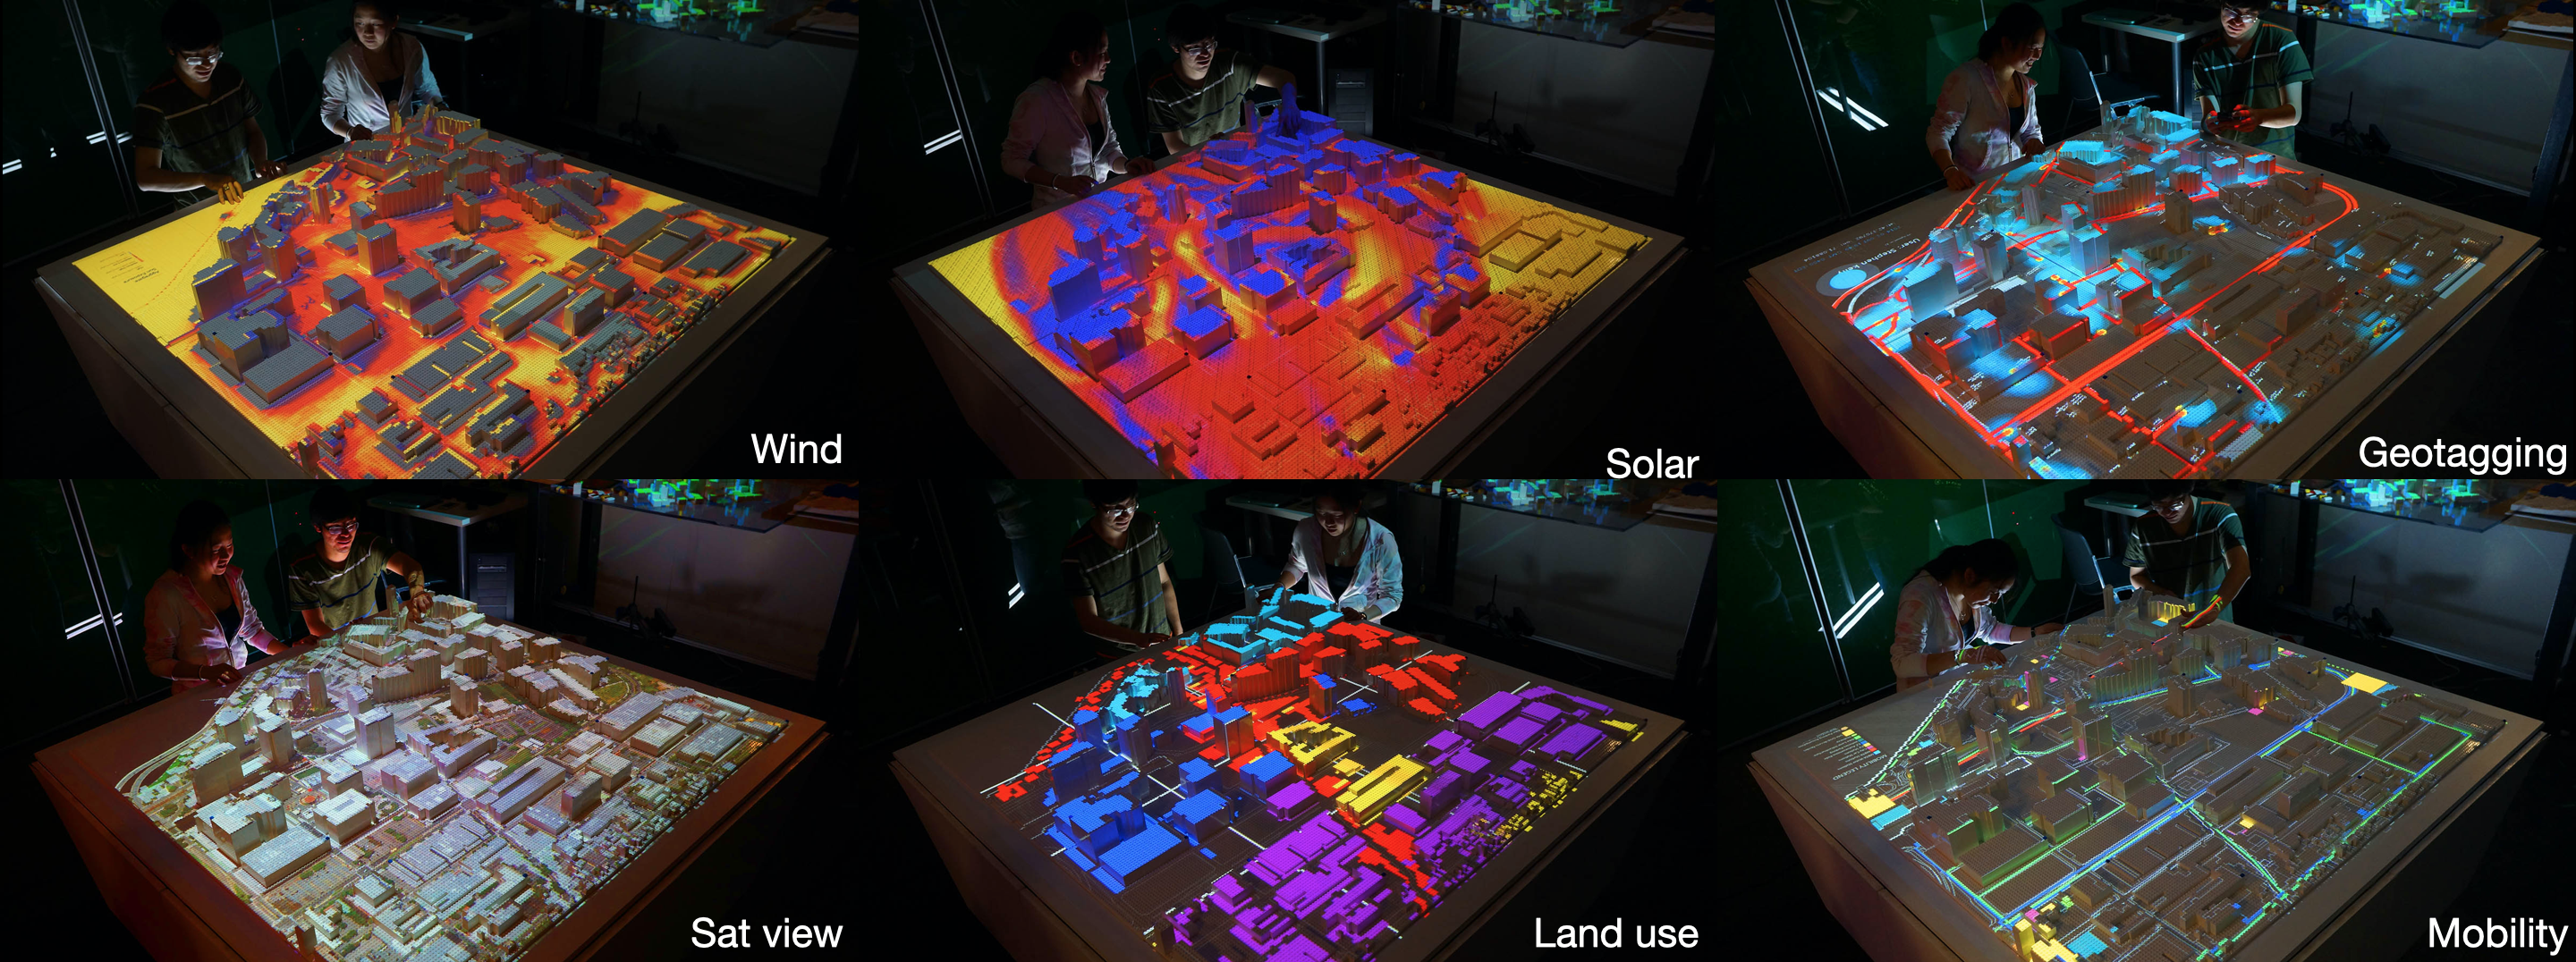
\includegraphics[width=1\textwidth]{chapters/insight/observatory/figures/urban_obs.png}
      \end{center}
      \caption{The Urban Observatory. Different layers of precomputed urban analysis projected onto a 3D model of the Kendall Sq. area in Cambridge, MA.}
      \label{fig:urban_obs}
  \end{figure}

  \subsection{System Design}
  {
      The Urban Observatory comprised of physical components, computer hardware, and custom display software, detailed bellow.

      \subsubsection{Computation}{\label{sec:computational-models}}
      {
          The Urban Observatory was design as an open canvas for displaying different layers of data, such as the formal properties of building designs, land-use, human activity and mobility, vehicular circulation, flows of energy, wind and solar exposure, and more (see Figure \eqref{fig:urban_obs}). These layers were pre-rendered in advance, since the platform was not set to perform spatial analytics or data acquisition in real-time\footnote{In later versions of CityScope, data for similar layers was fetched in real-time, and was rendered dynamically to reflect updated insights or user-interaction. See Chapter \eqref{ch:transformation}}. As part of the students' workshop, architectural, urban-planning, traffic-simulation, and visualization tools were all used to produce these data layers. The projection were projected and aligned to the 3D model using a Processing sketch \cite{reas2007processing}.
      }

      \subsubsection{Hardware}
      {
          The system contained two main elements: (i) a 3D urban model, made out of white LEGO bricks, and (ii) an array of overhang projectors. The physical model was of size $1.7m^2$, which represent a $1km^2$ area of Kendall Square, roughly as the scale of $4m$ for each LEGO stud. For projection, six video projectors were used: two to project the ground and roof planes of a physical model, and one projector for each of the four vertical surface orientations (north, south, east, and west), creating the illusion of 360$^{\circ}$ projection.
      }
  }

  \subsection{Usage}
  {
      The `Urban Observatory' was developed and situated in an active demonstration space at the MIT Media Lab building. Between '13-'16, hundreds of visitors, researchers, and students interacted with the installation; In 2015-2016, the platform was repurposed to support \textit{MAS.S65: The City Science Workshop}, an MIT course that was focused on prototyping new ways to collect and represent urban insights and spatial data. These insights were broad, and ranged from analyzing crime and energy, to vegetation and thermal comfort. Later that year, the 3D models was again repurposed to set as the base line for the CityScope Volpe project (see Section \eqref{sec:cityscope_volpe}).
  }

  \subsection{Discussion}{\label{subsec:observatory_discussion}}

  {
      The Urban Observatory was an early CityScope prototype, which projected pre-defined data layers and urban observations onto a tangible interface. Despite its simplicity, this prototype proven the advantage of merging spatial data and tangible interfaces, as a means to create a new `common ground' for urban discourse. This work also hinted to several features of future CityScope, such as: (i) A Data Warehouse that would store urban data, and spatial analytics algorithms (later to become cityIO, see Section \eqref{subsec:csarch-cityio}); (ii) User Interface, to provide a flexible and intuitive interaction for exploring different urban scenarios (such as CityScope TUI, see Section \eqref{subsec:mocho-volpe}); (iii) Interactive visualizations, to provide dynamic feedback to the users' design iteration (later to become CityScopeJS, see Section \eqref{sec:cityscope_architecture}). Arguably, the Urban Observatory's greatest contribution to the future of CityScope, was the idea of an open-ended urban `sandbox', on which new scenarios could be tested, and user contributions, feedback, and insights, would be collected.
      \newline
      As shown in the following work, later CityScope projects centered around behavioral, social, and economic insights, in order to look beyond the formal and physical aspects of the city.
  }
 }\label{sec:urbanobservatory}
%%%%%%%%%%%%%%%%%%%%%%%%%%%%%%%%%%%%%%%%%%%%%%%%%

\section{Urban Dynamics: CityScope Andorra}\label{sec:andorra-data-observatory-andorra}

{
    In 2014, the Andorran government and the MIT City Science group founded a `living lab' to prototype, deploy, and test urban innovation \cite{SmallEur15:online}. As part of this partnership, the Andorran Government promoted projects related to urban data collection and analysis, and supported this effort by sharing spatial, behavioral, and telecom data. Using these datasets, various research projects were proposed, including the analysis of tourism, mobility, urban-design, energy, environment, and public health \cite{9580719, Grignard:2018:CAM:3237383.3238030, leng2016analysis, noyman_inpress, doorley2020mpec}. The rest of this Chapter details case-studies that used these datasets for the purpose of gaining urban insights and supporting decision-making processes.
}
%%%%%%%%%%%%%%%%%%%%%%%%%%%%%%%%%%%%%%%%%%%%%%%%%
\section{(i) Andorra Data Observatory}\label{sec:andorra-data-observatory}
{
    As part of the collaboration with the Andorran government, a set of tools to analyze, visualize, and extract insights on large public events were create. This section details a data-visualization platform that (i) models the trajectories of large amount of individuals and visitors in several public gathering in Andorra's major cities, (ii) use Agent Based modeling (ABM) to analyze these patterns, and (iii) extract relevant insights and conclusions from these insights.

    \begin{figure}[h]
        \begin{center}
            \includegraphics[width=1\textwidth]{chapters/insight/and_abm/figures/and_cityscope.jpg}
        \end{center}
        \caption{CityScope Andorra at the City Science Lab in Caldea, Andorra la Vella. Built in 2016, this platform was one of the first to serve as an interactive, real-time tool for urban decision making. Here, a user interacts with a Tangible User Interface to asses the impacts of different interventions in the city center.}
        \label{fig:and_cityscope}
    \end{figure}

    \subsection{Events}
    {
        Andorra has a population of nearly eighty thousand, and hosts more than eight million visitors in a normal year, many of them as tourists\footnote{According to the \textit{Departament d\'Estad\'istica}, Andorra had approximately eight million visitors in 2016: 4.2M Spanish, 3.2M French, and 0.6M from other nationalities.}. The tourism sector accounts for $\sim$80\% of Andorra's GDP and thus large public events are critical for the local economy \cite{CIA}. This work focuses on observing the mobility patterns of both pedestrians and vehicles, as a product of tourists and visitors' attendance at annual events in Andorra. The work focuses on the following events: (i) \textit{Cirque du Soleil: VISION} and (ii) \textit{Le Tour de France}, both took place in 2016.
        \newline
        `Scalada' by \textit{Cirque du Soleil: VISION}, is a series of indoor, summertime shows, taking place between Tuesdays to Saturdays, July 2\textsuperscript{nd} - July 30\textsuperscript{th}, 2016. VISION's venue has a capacity for 5000 people per performance. \textit{Le Tour de France} is an annual multiple stage bicycle race held in France, which occasionally passes through nearby EU countries. In 2016, Andorra hosted \textit{Le Tour de France} Stage 9 in its mountain area (Arcal\'is, Ordino) as well as the departure of Stage 10 in the city center (Escaldes, Escaldes-Engordany).
    }

    \subsection{Data and Method}
    {
        Call Detail Records (CDR) are digital records gathered by the mobile network operator used for billing purposes. Observations are triggered by mobile phones actions such as phone calls, text messages, and cellular data. This source of data is broadly used in the research community, since it contains spatial information, allowing to conduct flow analyses \cite{Blondel2015, ccolak2015analyzing, Ratti2006}. As part of this work, Andorra Telecom shared nearly three years of CDR data (2014-2016)\footnote{In order to comply with privacy policies, all personal identifiers, such as names and mobile phone numbers, were anonymized based on a Secure Hash Algorithm (SHA-512), a one-direction encryption method preventing the retrieval of the information obscured.}. Each entry in the CDR contains unique anonymized caller id, the date and time of the call, call duration, and the id of the Base Transceiver Station tower, as shown in table \eqref{f:CDRSample}. with this data, tower-to-tower origin and destination matrices (OD) for each individual were computed.


        \begin{table}
            \begin{center}
                \begin{tabular}{c|cccc}
                    \hline
                    Anonymized ID & Call Date & Call Time & Duration & towerID \\
                    \hline
                    iAAJKnPAa5    & 20160716  & 09:34:13  & 18       & 2       \\
                    iAAJKnPAa5    & 20160716  & 10:21:43  & 156      & 6       \\
                    iAAJKnPAa5    & 20160716  & 13:02:37  & 38       & 10      \\
                    \hline
                \end{tabular}
                \caption{Sample of a CDR observation}
                \label{f:CDRSample}
            \end{center}
        \end{table}


        \subsubsection{Road Network}
        {
            CDR data provide scarce localizing per given user. The nature of these data dictates simplified tower-to-tower OD matrices that correspond to linear, non geographically accurate vectors. In order to correlate these trajectories to the existing road network, users are constrained to roam along a graph topology \cite{Gonzalez2008}. Roads of different types are set to bound different mobility modes (primary, secondary, residential, or pedestrian). In order to compute a more accurate shortest path, the road network is considered as a weight-directed graph used to constrain the behavior of users. The edge direction represents the directionality of the road; The weight combines the speed limit of the road and the number of user present on that road.
        }

        \subsubsection{POIs and Amenities}
        {
            Given the degree of noise in CDR data, urban amenities, such as restaurants, hotels, and other Points Of Interest, were used to anchor destination points of users. The geolocation of amenities was gathered using several public APIs, such as TripAdvisor and Yelp, as well as the \textit{Andorra Turisme} office.
        }
    }

    \subsection{System Design}
    {
        Processing the LBS dataset, and constraining the agents' movement to the road network and POIs, was done using GAMA, an Agent Based modeling (ABM) software \cite{grignard2013gama} and Processing \cite{reas2007processing}. Using a Tangible User Interface (TUI), users could interact with the simulations, and trigger different visualization layers. The three main classes in the model are an abstraction of the (i) environment (cell towers, roads, and amenities), (ii) mobile agents (people and vehicles), and (iii) interactive grid. The rest of this section details the implementation of the ABM and the visualization of the results on a TUI.

        \begin{figure}[h]
            \begin{center}
                \includegraphics[width=0.4\textwidth]{chapters/insight/and_abm/figures/and_cdr_arch.png}
            \end{center}
            \caption{CityScope Andorra data pipelines and TUI. The ABM is computed from both static (GIS) and dynamic (telecom) datasets. It reacts to changes occurring on auxiliary interfaces (CityScopeAR, CityMatrix) and recompute the simulation in accordance.}
            \label{fig:and_cdr_arch}
        \end{figure}


        \subsubsection{Agent Based Model}
        {
            The ABM uses several datasets to characterize agents' behavior in the city: (i) telecom data, (ii) road network, and (iii) amenities and POIs data.
            \newline
            \textbf{Agents:} The virtual environment (`world') is populated with independent agents, each with an assigned set of variables that influence their behavior whenever changes occurs, either locally or at the surrounding environment. \textbf{State:} The agent's variables are (1) agent's country of residence; (2) origin location: defined using telecom data; (3) preferred destination, generated by predefined or dynamically added urban anchors; (4) distance traveled; (5) speed of movement; and (6) passable network nodes. \textbf{Behavior:} The agent's trajectory is determined by the OD matrix computed from the CDR data. The path is computed by constraining the OD to the local road network. The agent's destination is anchored to the amenity closest to the cell tower coverage where its action was recorded when terminated. The chosen amenity depends on the agent's country of residence and the language affinity of the amenities. Depending on its speed (time difference between origin and destination location), the agent will be considered as a pedestrian (solid circle) or as a vehicle (stroke circle).
            \newline
            Agents can adapt themselves to several dynamic factors: (i) traffic congestion: in case of severe congestion, a pathfinding method is called to recalculate an alternative route. If a road is busy, the agent will recompute a shortest path to its destination in order to avoid that road; and (ii) amenity occupancy: if the amenity assigned as destination is flagged as full, the agent can select another amenity close-by to its prior destination. Once agents reach their destination, they stay there for a few iterations. The number of iterations is defined by the average time spent on those places, retrieved from the different APIs.
        }

        \subsubsection{Visualization}
        {
            The ABM was displayed via three main visual layers: (i) Spatial elements, such as geography, buildings, amenities, cell towers, and roads, (ii) Pedestrian and vehicular movement from the ABM, and (iii) Amenities' popularity and density. Pedestrians were represented by solid circles and vehicles by stroke circles, colored according to their origin country: Orange refers to visitors from Spain, blue for France, and white for other countries\footnote{This classes were suggested by \textit{Departament d'Estad\'itica d'Andorra}, although the telecom data has more detailed classification via the IMSI property}.
            The visual representation of POIs and amenities echos the number of agents currently resting at a given location, indicating the activity level in a place. The large white circle highlights the location where the show was taking place. The simulation concluded that 5,174 visitors attendees at the same time, within a reasonable range of \textit{Andorra Turisme} official tally of 4,540 visitors.
            \newline
            Unlike \textit{Cirque du Soleil}, \textit{Le Tour de France} is an outdoor event in which no ticketing process can help assess attendance. Therefore, an aggregated heatmap representation was used to summarize global activity, and provide geo-located attendance estimates. Figure \eqref{fig:and_cdr_viz} show occupancy levels for \textit{Le Tour de France} during July 12\textsuperscript{th}. The race starting point was at Escaldes-Engordany, shown as the most active area in Figure \eqref{fig:and_cdr_viz}, with large concentration on the left side.

            \begin{figure}[h]
                \begin{center}
                    \includegraphics[width=1\textwidth]{chapters/insight/and_abm/figures/and_cdr_viz.png}
                \end{center}
                \caption{
                    (top left) Aggregated congestion for the entire day during \textit{Le Tour de France}. (top right) Travel patterns anchored to the road network and associated to inferred amentias as destination points. (bottom left) Raw CDR data; points represent locations recorded from cell towers. (bottom right) `Hot-spots' agglomerated in areas where multiple simulated agents are passing through a given street.
                }
                \label{fig:and_cdr_viz}
            \end{figure}
        }

        \subsubsection{Tangible Layer}
        {
            \begin{figure}[h]
                \begin{center}
                    \includegraphics[width=1\textwidth]{chapters/insight/and_abm/figures/trajectory.png}
                \end{center}
                \caption{Trajectories are computed by traversing between the CDR records, and aligning the trip to existing road network. The speed between these points is assumed to be a proxy for mode of transit (faster=car/transit, slower=bikes/foot).}
                \label{fig:and_trajectories}
            \end{figure}

            The Andorra CityScope TUI has three components: (i) A physical 3D model of the city made out of LEGO, (ii) An abstract representation of a redevelopment area at the city's center, and (iii) Augmented Reality (AR) data-visualization system.
            \newline
            In 2016, a physical model was built, consisting of a 3D topographical model of the two main cities in Andorra: Andorra la-Vella and Escaldes-Engordany. The outskirts of these two cities, as well as cities located near the border (Sant Julia de L'oria near the Spanish border and Pas de la Casa near the French border) and the parishes of Canillo, Encamp, Ordino, and La Massana, are abstractly represented using pie-chart like population clusters. A temporal indication of the visitor's flow is displayed using a slider, and the population volume is displayed by a histogram.
        }

        \subsubsection{Augmented Reality}
        {
            \begin{figure}[h]
                \begin{center}
                    \includegraphics[width=1\textwidth]{chapters/insight/and_abm/figures/and_ar.jpg}
                \end{center}
                \caption{CityScopeAR: Augmented reality platform for CityScope Andorra. Remote participation and complex 3D visualizations are extending the capability of CityScope beyond the limitations of the physical TUI.}
                \label{fig:and_AR}
            \end{figure}

            An Augmented Reality subsystem was designed to allow users to observe spatial, ABM, and interventions data using different devices, client-side applications, web-based interfaces, AR, or VR \cite{noyman2018CityScopeARUD} (for a detailed breakdown of the CityScopeAR system see Section \eqref{sec:cityscope_ar}). The AR subsystem collects data from several sources: (i) Raw telecom data (CDR OD matrix), (ii) Existing built environment, (iii) Real-time 3D representation of design and planning iterations, and (iv) Mobility analysis. In the use-case of Andorra, which is poised in the heart of a sensitive natural landscape, any urban intervention might have major spatial impacts (see Figure \eqref{fig:and_AR}). It is therefore crucial to understand how changes might affect urban form, usability, access, and land-use patterns ahead of urban transformation. The AR layer worked in concert with the TUI, so that users could better sense the spatial implications of urban interventions (see in detail \eqref{ch:transformation} and \eqref{sec:cityscope_ar}).
        }
    }

    \subsection{Discussion}
    {

        \begin{figure}[h]
            \begin{center}
                \includegraphics[width=1\textwidth]{chapters/insight/and_abm/figures/and_cs_ppl.jpeg}
            \end{center}
            \caption{CityScope Andorra at the City Science Lab in Caldea, Andorra la Vella. The space is situated in the heart of the city, and was designed to accommodate multi-party discussions, meetings, and events, around a large scale CityScope installation.}
            \label{fig:and_cityscope_ppl}
        \end{figure}


        The Andorra Observatory was developed at MIT (`16-`17), deployed at the Barcelona Smart City Expo World Congress, and was finally mounted in Andorra in late 2017. It was on display in dozens of public demonstrations, and was viewed by thousands of visitors, both at MIT, the City Science Lab in Andorra la-Vella, as well as in the Barcelona Expo in 2016.
        \newline
        The Andorra Observatory was designed to provide a comprehensive view of the city's activity and mobility, and to allow users to interact with the ABM through TUI and AR. The underlining ABM use of CDR data demonstrated the ability to visualize the city's activity and mobility at both local and global levels. As shown in the the rest of this Chapter, the incorporation of better location, spatial, and demographic data can improve the accuracy of such models and the quality of urban insights.

    }
}

\label{sec:and_abm}
%%%%%%%%%%%%%%%%%%%%%%%%%%%%%%%%%%%%%%%%%%%%%%%%%
%%%%%%%%%%%%%%%%%%%%%%%%%%%%%%%%%%%%%%%%%%%%%%%%%%%%%%%%%%%%%%%%%%%%%%%%%%%%%%%%
\section{(ii) Urban Performance Inference with Telecom Data}

 {
  Following the work done using CDR data\footnote{see Section \eqref{sec:andorra-data-observatory}, and references \cite{leng2016analysis, grignard2017agent}}, the Andorran Government offered several new data pipelines containing high resolution location data. Radio Network Controller (RNC), a statewide location data source became available for multiple periods between 2015-2021. Using RNC, two statistical models were developed to explore the relationship between the physical features of Andorran cities and the discrete behavior of its residents and visitors. These models highlighted various dependencies and detractions between certain urban-design settings, and human behavioral patterns. This study suggests a method of statistical analysis to evaluate the performance of public spaces, as a proxy of the prevalence of certain behaviors to occur.
 }

\subsection{Introduction}

{
    Vibrant public spaces that attract dense and diverse populations, are an integral part of any successful urban district \cite{krier1979urban, banerjee2011companion, gehl2013study}. Nevertheless, accurate correlation between public spaces and human activity is hard to measure and analyze \cite{gehl2013study, Calabrese2014}. In recent decades, data-driven methods for the analysis of urban places, became possible using Location-Based Services and new statistical processing techniques \cite{Hillier1993}.
    This work marries a high-resolution location dataset, and a set of urban properties, to infer the relationships between human behavior and spatial arrangement of public spaces. The rest of this section details the site and data used in this work.

    \subsubsection{Study Area}
    {
        The city center of Andorra is located in a steep Valley made by the Valira river (100m - 600m width). This topography formed an organically shaped urban-center that merges with its natural surroundings. Andorra has no airport or train service, so that the majority of nearly 8 million visitors per year arrive by motorized vehicles from either Spain or France \cite{CIA}. Both Andorra La-Vella and Les Escaldes municipalities were considered in this study.
    }

    \subsubsection{Data}
    {
        Andorra Telecom (AT), the sole telecoms service in Andorra, provided the data for this study. Having a singular country-wide telecom provider, differentiates this dataset from those acquired in other cities, where a fragmented market usually holds multiple cellular providers \cite{louail2014mobile}. The third generation (3G) network operated by AT is a Universal Mobile Telecommunications System (UMTS) network and the governing element of the UMTS network is the Radio Network Controller (RNC) \cite{ETSI}. One function of the RNC is to keep track of the locations of devices as they move around the coverage area, without the need for an active device usage. Each time a connected device interacts with the network (through call, text or cellular data), moves from one cell tower to another, or goes unobserved for more than 90 minutes, an observation is recorded. Each observation includes a unique id for the subscriber, a timestamp, the device coordinates at the time of the update, and the home network of the subscriber. The coordinates are given in the standard WGS84 system, estimated by AT to be within 25-100m in urban areas, significantly more precise than Call Detail Records (CDR) \cite{gonzalez2008understanding, Deville2014, blondel2015survey}. AT utilizes enhanced triangulation using the angle, time and RSS received by the device from different base-stations, as well as error mitigation using a proprietary algorithm. For the purpose of the study, data from Saturdays in September 2016 were used. Only Saturdays were considered, in order to focus on social activity rather than work activity, and the two days chosen were ones without any large cultural events which could create anomalies.
    }
}

\subsection{Methodology}
{
    In order to model the relationship between human activity and urban-design, two pre-processing steps were taken: (i) The aggregation of human behavior into clusters, and (ii) the agglomeration of urban features, POIs, and amenities, as explanatory variables. This Section describes these pre-processing steps.
}

\subsubsection{Stay-events and Activity Clusters}
{

    \begin{figure}[!h]
        \begin{center}
            \includegraphics[width=1\textwidth]{chapters/insight/revurb/figures/revurb_data.png}
        \end{center}
        \caption{Stays and Cluster. (left) Stay events analysis over 24hrs duration and the DBSCAN method which extracts clusters. (right) clusters culling based on `persistance', which is the duration a moving cluster sustain throughout the day.}
        \label{fig:revurb_data}
    \end{figure}

    In this work, urban behavior is evaluated through the formation of dense clusters of non-transient activity. These clusters are considered to be important as they allow to identify not only those places in which individuals spend time, but the places where diverse groups of people congregate together, creating the potential for social interaction. The identification of activity clusters is carried out by a 2-step procedure: (i) finding stay-points and (ii) clustering those stay-points with certain parameters. The overall process is illustrated in Figure \eqref{fig:revurb_clusters}.
    \newline
    \textbf{Stay-events:} The purpose of the first step is to eliminate `roaming' observations (i.e., where a person is only passing through an area), and retain only events where a person has intentionally stayed in a particular vicinity for a certain amount of time. A stay-point is defined as a group of observations of a person's location, whereby no point is greater than 200m from any other point and the time elapsed is at least 20 minutes \cite{li2008mining}. The maximum distance and minimum time parameters were considered appropriate as they would filter out common roaming events, while preserving activities for which this particular location has been chosen.

    \begin{figure}[!h]
        \begin{center}
            \includegraphics[width=0.75\textwidth]{chapters/insight/revurb/figures/revurb_clusters.png}
        \end{center}
        \caption{Clustering stay-points as `Moving Clusters'. Each potential cluster was deemed relevant considering its longevity, density, and diversity. The map show clusters formed near the city-center.}
        \label{fig:revurb_clusters}
    \end{figure}

    \textbf{Clusters:} Following the identification of individual stay-points, a density based clustering algorithm was used in each 10-minute time period to find locations where groups of individuals congregate together. Such algorithms agglomerate some points to clusters while leaving other points un-clustered, so that the density of stay points within the clusters is considerably higher than the density of points outside of the clusters. The clustering algorithm is Density-Based Spatial Clustering of Applications with Noise (DBSCAN) \cite{ester1996density}, which is capable of efficiently finding clusters of arbitrary shape, size and quantity\footnote{DBSCAN is based on the notion that the density of a point in a dataset is a function of its spatial-temporal proximity to other points in the dataset, hence it overcome clustering issues that appear in other methods, such as K-means or PCA \cite{ester1996density}.}. In relating the clusters to urban features, each cluster was represented by its centroid; Since individual RNC observations had a standard error of ~50m, the coverage region of the cluster could not be known with enough precision. However, the standard error of the cluster centroid decreases with the number of observations, making this estimate much more reliable.
    \newline
    \textbf{Findings:} Some insights could already be gained from observation of the produced clusters, prior to any model fitting: Clusters tended to form along the main river passing through the city, as well as near commercial centers, including `Leclerc' supermarket, and cultural museums, such as Natural History Museum and Carmen Thyssen Museum. On the contrary, clusters were less likely to form around big urban green spaces and sparsely built environments. These insights are expected, given the tendency of human activity to form along geographical features, leisure places, and amenities. Nevertheless, the goal of this study was to provide a high-resolution explanatory model that can show which urban features and their agglomeration are highly correlated with clusters of activity.
}

\subsubsection{Identifying Urban Features} \label{subsec:urbFeat}

{
    \begin{figure}[!h]
        \begin{center}
            \includegraphics[width=0.75\textwidth]{chapters/insight/revurb/figures/revurb_features.png}
        \end{center}
        \caption{Urban features, temporal data and the city. Isometric view of the different datasets and urban features used in this study. Purple layers represent static data, and pink layers represent temporal and dynamic observations.}
        \label{fig:revurb_layers}
    \end{figure}

    In order to relate the activity clusters to spatial features, a set of candidate features was proposed. This list considered core elements of the public realm, such as transportation networks, landscape elements, or commercial buildings, which might be more likely to influence the creation of activity clusters. These correspond to classic urban theories, such as the five elements of mental maps \cite{lynch1960image}, the pattern languages \cite{alexander1977pattern}, as well as contemporary urban-design evaluation frameworks \cite{hassan2014evaluation}. Included in the feature set were locations of amenities from the Google Places API, as well as bus stops, GIS shape files of buildings, roads, green spaces, water features and car parks from OpenStreetMap \cite{haklay2008openstreetmap}. Figure \eqref{fig:revurb_layers} shows the various stages of processing the RNC data along with the categories of urban features considered in the model fitting. Appendix Table \eqref{tab:andorra_model_features} lists the features considered in the model fitting.
}

\subsubsection{Subdivision of Study Area}
{
    In this study, a single measure of behavioral pattern (clusters) and the associated set of urban features (form, function, or morphology) would constitute a single observation. However, as in many other instances of spatial analysis, the observed data is based on events occurring in continuous space and time, and therefore do not naturally form such a structure. For this reason, it is common to subdivide the study area into spatial polygons with defined boundaries; These polygons are then used as bins to aggregate the observed data into discrete observations \cite{bivand2008applied}.
    \newline
    In the case of Andorra's physical formation, no obvious morphological tessellation of the study region was apparent. The natural landscape formed by the Pyrenees mountains forced an organic urban form to evolve, making urban blocks or road network grid unconstrained enough for analysis. As shown in the upper part of Figure \eqref{fig:revurb_layers}, the city center of Andorra was instead divided into a regularly spaced grid of $50mx50m$ cells. The size of the cells was chosen in order to be at the scale of the urban features, as well as within the bounds of the telecom data accuracy threshold\footnote{At an early stage of this work, a 25sqm grid was attempted but resulted in a lower model fit.}. All of the behavioral and urban feature metrics were computed for every grid cell in the study region, 962 in total.
}

\subsection{Models}
{

    The location data was preprocessed through DBSCAN, an unsupervised clustering algorithm, in order to groups together activities across time and space. Following the clustering, two methods were developed to examine the relationship between human behavior, and the usage patterns of urban feature:
    \newline
    (i) The first uses two supervised learning algorithms, \textbf{Multivariate Linear regression} (MLR and Lasso MLR), which were fit to the clusters in order to asses total clustering population, normalized clustering time and clustering diversity, and suggest which amenities are more representative for the creation of these clusters.
    \newline
    (ii) The second model is based on \textbf{Inhomogeneous Poisson Process (IPP)}, a density based clustering algorithm, where the density of a process varies in space in association with the urban features. The IPP intensity was found to be positively associated with amenities such as shopping and entertainment, the availability of parking and bus stops and the presence of natural water features. The intensity was negatively associated with the distance from the city centre and streets and with presence of hotels.
    \newline
    Both models are detailed in the following sections.
}

\subsection{(i) MLR and Lasso Regression}
{
    The first modeling method uses two flavors of regression models: Multivariate Linear Regression (MLR) and Lasso Multivariate Linear Regression (Lasso). Results from both methods are included in this study as MLR provides intuitive results which include p-values, whereas lasso MLR provides additional validation to the results \cite{neter1996applied}\footnote{See Appendix Section \eqref{appendix:mlr_and_lasso_mlr} for more on the differences and advantages of using both methods}.

    \subsubsection{MLR Model Training}\label{mlr_model_training}
    {
        Three variants of this model were fit to the data: (i) total clustering population, (ii) normalized clustering time, and (iii) clustering diversity. In order to identify the best fitting model, a forward stepwise search was carried out from the null model to a model including all variables. At each step, a single variable was chosen to be added to the model based on how much it would improve the Akaike Information Criterion (AIC) of the model. If there were no variables remaining whose addition to the model would include the AIC, the stepwise search concluded with the current model.
    }

    \subsubsection{MLR Results}
    {
        Over a period of 16 days (between Sept. 15 - 30, 2016) 2,422,065 stay-points and 10,908 moving clusters were identified. The results of the model fitting process are presented in table \eqref{tab:mlr-results}:
    }

    \begin{table}
        \caption{Model results. (N: Number, B: Binary, I: Index, MSE: Mean squared error, CV: Cross validation, SE: Standard Error)}
        \begin{center}
            \begin{tabular}{l|llcl}
                \multirow{2}{*}{\textbf{\begin{tabular}[c]{@{}l@{}}Variable:\\ Services {[}N{]}\end{tabular}}} & \multicolumn{3}{l}{\textbf{Multivariate Regression}} & \textbf{Lasso}                                                  \\
                                                                                                               & \textbf{Coefficient}                                 & \textbf{p-value} & \textbf{Significance} & \textbf{Coefficient} \\

                \noalign{\hrule height 0.25pt}
                Size                                                                                           & 0.15                                                 & 4.84E-11         & ***                   & 0.12                 \\
                Persistence                                                                                    & 0.31                                                 & 6.40E-10         & ***                   & 0.27                 \\
                Diversity                                                                                      & 0.28                                                 & 0.00678          & **                    & 0.22                 \\
            \end{tabular}
        \end{center}
        \label{tab:mlr-results}
    \end{table}

}


\subsection{(ii) Point Process Model} \label{sec:ppm}

{
    The second modeling method is a Point Process Model. This approach is a better fit for events distributed over time and space, such as the clustering of time-series stay-points and urban features. A point process is a stochastic mechanism that generates a countable set of events inside a region of space \cite{diggle2013statistical}. Occasionally, a point process may exhibit Complete Spatial Randomness (CSR). In such cases the process may be modelled as a Homogeneous Poisson Process \cite{baddeley2008analysing}. This model describes the expected number of points, \textit{P}, found in any arbitrary window \textit{B} as
    $
        \mathbb{E}[count(P \quad in \quad B)] = \lambda \times area(B)\inlineeqno{(1)}
    $
    where $\lambda$ is the intensity of the process. Homogeneous Poisson Processes are rarely used in practical applications, as most point patterns have intensity which varies in space, often in association with one or more covariates. In this case, the process may be modelled as an Inhomogeneous Poisson Process (IPP). This model describes the expected number of points found in any arbitrary window as
    $
        \mathbb{E}[count(P \quad in \quad B)] = \int_{B}\lambda(u)du \inlineeqno{(2)}
    $
    where the intensity $\lambda$ is a function of the covariates $x_1(u)$ to $x_n(u)$.
    $
        \lambda(x)=\exp(\beta_0+\beta_1x_1(u)+\beta_2x_2(u)+...)\inlineeqno{(3)}
    $
    All clusters found over the data duration were aggregated to form a 2-dimensional point-pattern in continuous space throughout the study region. The Inhomogeneous Poisson Process (IPP) is used to model the occurrence of activity clusters as a function of the set of urban features described above.
    \newline
    In order to include urban features as covariates in the IPP model, they must each be represented as a 2 dimensional image. For the point features, which included locations of amenities and bus-stops, kernel-smoothed densities were used. The kernels were all Gaussian with a standard-deviation of 20m. For the polygon features such as buildings, binary masks were used. The IPP model can be fitted to the data by maximizing the log-likelihood function using the Berman-Turner algorithm \cite{berman1992approximating}.
    The fitting process was carried out using the \textit{R} computing software using the \textit{spatstat} package \cite{baddeley2005spatstat}. Each of the features described in section \eqref{subsec:urbFeat} was considered for inclusion in the model. As with the MLR model, in order to prevent model over-fitting, a forward step-wise selection procedure was used \cite{friedman2001elements}. An advantage of this method is that a fitted IPP model can be used to simulate new sets of cluster locations for any other similar region, where the urban features can be similarly measured.
}

\subsection{Results and Discussion}
{


    \begin{figure}[!h]
        \centering
        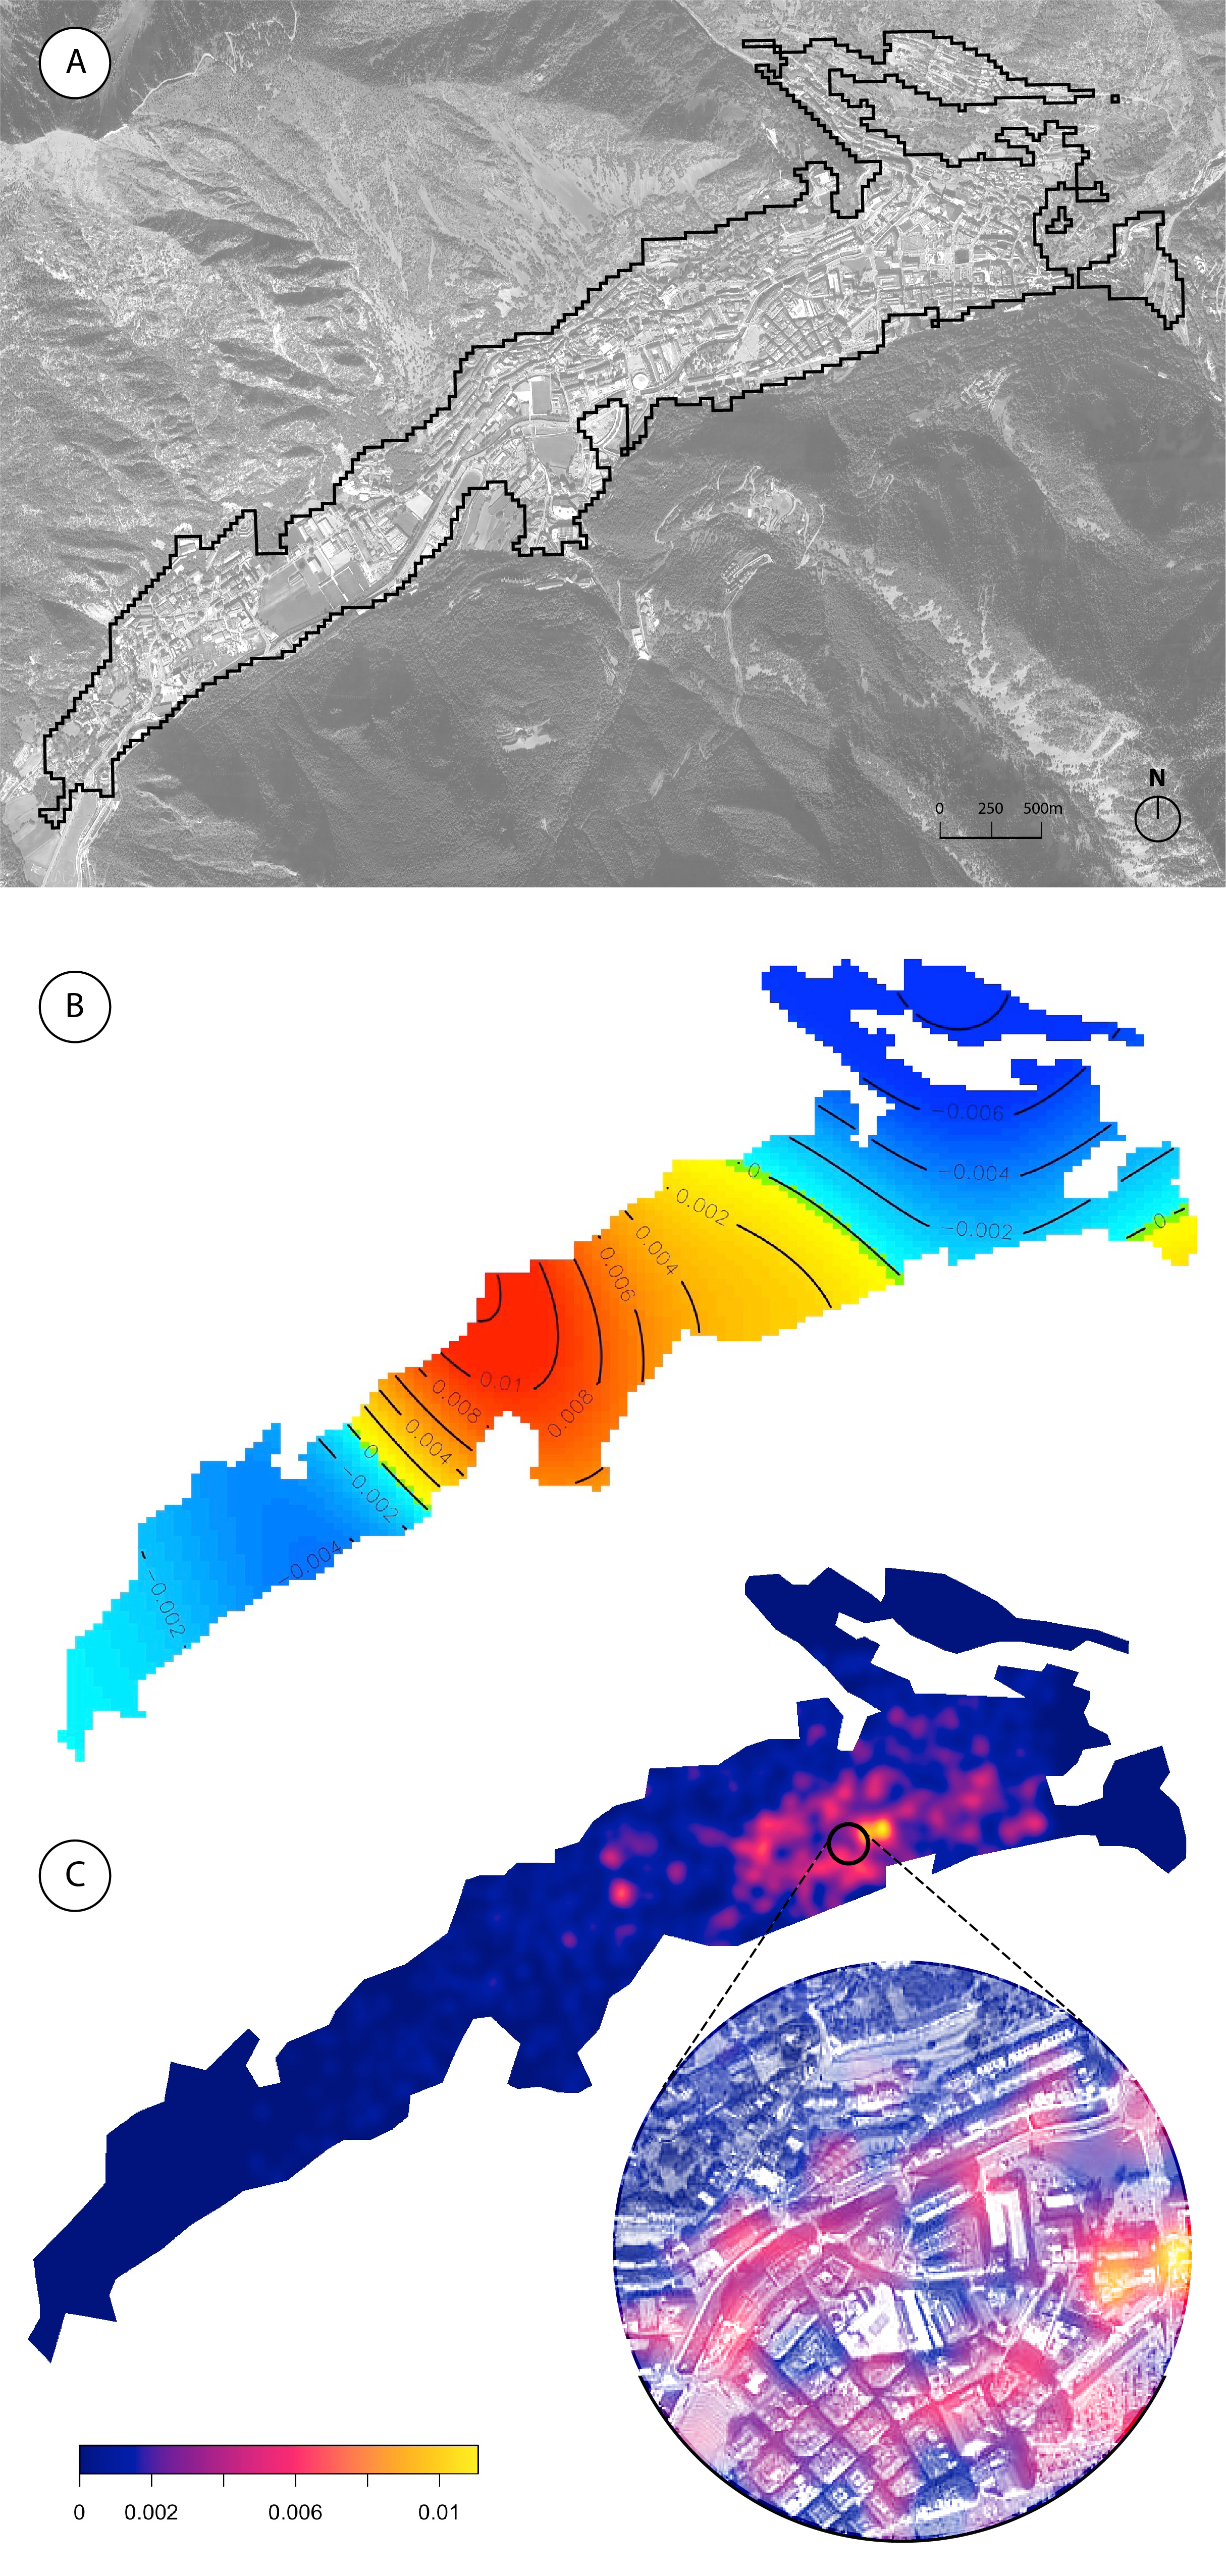
\includegraphics[width=0.5\textwidth]{chapters/insight/revurb/figures/revurb_ppm.jpg}
        \caption{Model area and densities. (a) Study region, (b) Contour plot of Pearson residuals from fitted model, (c) Smoothed density of points simulated from Inhomogeneous Poison Process model}
        \label{fig:ppm_res}
    \end{figure}

    The step-wise selection procedure outlined in Section \eqref{sec:ppm} resulted in a model which included 14 of the 16 urban features considered. The only variables excluded due to their failure to improve the AIC were Food and Education amenities. The coefficients of included variables and their significance levels are presented in Table \eqref{tab:results}.

    \begin{table*}[!h]
        \centering
        \caption{Results of Model Fitting}
        \label{tab:results}
        \begin{tabular}{ c|cccc }
            \hline
                       & Feature                & Estimate & Standard Error & Significance \\
            \noalign{\hrule height 0.5pt}
                       & (Intercept)            & -6.33    & 0.08           & ***          \\
            Amenities  & Entertainment          & 2552.53  & 302.75         & ***          \\
                       & Government             & 1068.22  & 235.25         & ***          \\
                       & Hotel                  & -1303.1  & 201.03         & ***          \\
                       & Religion               & 1191.52  & 424.82         & **           \\
                       & Service                & 827.62   & 39.79          & ***          \\
                       & Shopping               & 160.18   & 15.12          & ***          \\
                       & Car Parks              & 1.15     & 0.06           & ***          \\
                       & Bus Stop               & 2030.52  & 187.35         & ***          \\
            Distances  & d\_Motorized\_Streets  & -0.01    & 0.001          & ***          \\
                       & d\_Pedestrian\_Streets & -0.001   & 2.7E-4         & ***          \\
                       & d\_City\_Center        & -7.9E-4  & 4.5E-5         & ***          \\
            Urban Form & Water                  & 1.22     & 0.08           & ***          \\
                       & Green Space            & -14.34   & 202.56         &              \\
                       & Buildings              & 0.13     & 0.05           & **           \\
            \hline
        \end{tabular}
    \end{table*}

    The kernel smoothed density of a point pattern simulated from the model is provided in Figure \eqref{fig:ppm_res} (c). A 3-dimensional contour plot is also provided in
    Figure \eqref{fig:ppm2} to illustrate how the model could be used to graphically depict the expected density of social activity in an urban district.


    \begin{figure}[!h]
        \centering
        \includegraphics[width=0.6\textwidth]{chapters/insight/revurb/figures/revurb_ppm2.jpg}
        \caption{Perspective contour plot of point pattern simulated from Inhomogeneous Poison Process model}
        \label{fig:ppm2}
    \end{figure}


    \subsubsection{Validation and Predictabilty}
    {
        Validation of the IPP model can be done using both formal and informal methods. The likelihood ratio test is an appropriate formal method for Poisson processes \cite{baddeley2006modeling}. This can test the null hypothesis of a Homogeneous Poisson Process in favour of the alternative hypothesis of an Inhomogeneous Poisson Process with intensity that is a log-linear function of the final set of features. An extremely small p-value is found for the final model in this study, indicating that the null hypothesis should be rejected in favour of this model. The informal methods involve visual inspection of the model residuals.
        \newline
        Figure \eqref{fig:ppm_res} (b) shows a contour map of the residuals of the final model. This plot indicates that, despite the high statistical significance of the features included in the model, there are still some areas of the urban district where intensity is over-predicted and other areas where it is under-predicted. This suggests that there are some features missing from the model which could improve predictive power. Nonetheless, since many of the features which were included were strongly associated with cluster intensity, valuable insights about urban behaviors can still be gained from this model.
    }

    \begin{figure}[!h]
        \begin{center}
            \includegraphics[width=1\textwidth]{chapters/insight/revurb/figures/revurb_cell_results.jpg}
        \end{center}
        \caption{Model inference on a single grid-cell. The urban features are highlighted on the left, with their modelled coefficients on the right.}
        \label{fig:revurb_cell_results}
    \end{figure}

    \subsubsection{Results and Insights}

    {
        A number of key insights could be drawn form the fitted models. First, certain amenities were associated with clustering intensity with high statistical significance. In particular, bus stops, car parks, and amenities categorized as Entertainment, Government, Religion, Service and Shopping were positively associated with clustering. The only type of amenity which was negatively associated with clustering was Hotels. Clusters were much more likely to occur closer to the city centre and closer to roads, both motorized and pedestrianized. Of the urban form elements, both natural water elements and buildings were positively associated with clustering.
        \newline
        Perhaps most surprisingly, green spaces, which are commonly perceived as desired public spaces for diverse and long-lasting gatherings, were negatively associated with clustering; This association was not statistically significant but the variable was included in the model as it improved the AIC. This detraction pattern might be explained by the definition of clusters based on density: Although parks and other green spaces are typically popular places for people to stay, the concentrations of people can be expected to be sparser than, for example, the confines of a shopping street.
    }
}

\subsection{Discussion}
{
    This study has demonstrated a methodology for assessing the performance and degree of activity of urban spaces, given spatial and telecoms data. The methodology found statistically significant associations between several types of urban features and the tendency for activity clusters to form around them. The rest of this section will discuss the contribution, potential, and limitations of this work.

    \subsubsection{Limitations}
    {
        The region and time period covered by the RNC dataset were relatively small, making this study's result less generalizable. Moreover, differences in culture, geographical, and seasonal factors might produce different outcomes when applying this method to other regions. The data used were of high resolution compared to many urban studies \cite{Louail2014} but the resolution was still not high enough to infer, for example, usage of specific amenities by individuals. As well, the RNC dataset is subject to propitiatory and commercial restrictions; This prevents the data and the full details of the underlying algorithm to be publicly available. Lastly, while the model results showed that many of the considered urban features were statistically significant with respect to behavior, the residual plot revealed partial spatial correlation, indicating that certain features might be missing from the model.
    }

    \subsubsection{Contribution and Opportunities}

    {
        The main contribution of this work is in providing a methodology that can be used in an evidence-based city-planning process. Using this approach, planning actions could be evaluated based on their likelihood to encourage vibrant social activity or - if desired - the lack of it. Even if the model predictions may not be precise in terms of the exact locations and sizes of activity clusters, the effects of each type of feature can be accurately predicted in terms of direction and relative effect size. With more accurate data and more robust models, this approach could be used to hint to the effectiveness of future urban-design interventions, especially in `infill' projects.
        \newline
        Finally, this work demonstrated the potential of spatio-temporal data to be used for gaining high-resolution insights. In an evidence-based urban process, these insights can help assess the impacts of spatial interventions on human behavior, and thus the effectiveness of proposed interventions. As Chapter \eqref{ch:prediction} entails, these type of implicit models could be used to help forecast the likelihood of a certain action to occur or to change in accordance with urban transportation.
    }
}





\label{sec:revurb}
%%%%%%%%%%%%%%%%%%%%%%%%%%%%%%%%%%%%%%%%%%%%%%%%%


%%%%%%%%%%%%%%%%%%%%%%%%%%%%%%%%%%%%%%%%%%%%%%%%%%
\section{Discussion: From Data to Actionable Insights}

 {
  This Chapter discussed the potential of urban insights to inform decision-making in planning, mobility, energy, tourism, and other aspects. While some insights could be gained from viewing a narrow perspective of the city, more advanced urban insights are the product of superimposing many different observations and data layers, so that anomalies, edge-cases, and relevant questions would arise. If done right, insights are a powerful tool to initiate urban decision-making, and can begin to inform the development of urban policies, strategies, and counterfactual scenarios. Importantly, real-time and updated insights can reduce the risks associated with asynchronous planing processes, in which by the time development has started, the state of the city has already changed.
  \newline
  The next Chapter explore ways to utilize such insights in the process of transforming the built environment.
 }


